\begin{appendices}

\chapter{Appendices}
\label{ch:appendices}

\section{Appendix A - Deployment Roles \& Users}
\label{appendix:roles_users}

\Cref{fig:appendix_roles_users} presents the identified user roles of the \acrfull{dcs} in red, to the left, and the identified users in blue, to the right. Also see (Electronic Appendix \ref{appendix:e_roles_users}).

\begin{figure}[htp]
    \centering
    \label{fig:appendix_roles_users}
    \includegraphics[width=\linewidth]{appendices/mind_maps/ABE_Users_slides_Oct26.pdf}
    \caption{Mind Map representing the different users \& roles identified for a \acrshort{dcs} deployment.}
\end{figure}

\section{Appendix B - Environment Attributes}
\label{appendix:environments}

\Cref{fig:appendix_environments} presents the identified environment attributes for the \acrfull{dcs}. Also see (Electronic Appendix \ref{appendix:e_environments}).

\begin{figure}[htp]
    \centering
    \label{fig:appendix_environments}
    \includegraphics[width=\linewidth]{appendices/mind_maps/ABE_Environments_slides_Oct26.pdf}
    \caption{Mind Map representing the different environment attributes identified for a \acrshort{dcs} deployment.}
\end{figure}

\section{Appendix C - System Use Cases}
\label{appendix:use_cases}

\Cref{fig:appendix_use_cases} presents the identified use cases for the \acrfull{dcs}. Also see (Electronic Appendix \ref{appendix:e_use_cases}).

\begin{figure}[htp]
    \centering
    \label{fig:appendix_use_cases}
    \includegraphics[width=\linewidth]{appendices/mind_maps/ABE_Use_Cases_slides_Oct26.pdf}
    \caption{Mind Map representing the different use cases identified for a \acrshort{dcs} deployment.}
\end{figure}

\section{Appendix D - Enrolment Diagram for Staff User}
\label{appendix:enrolment_diagram}

\Cref{fig:appendix_sta_deployment} represents a deployment diagram for the \theResServer system, with staff member enrolling into the system. This diagram is an alternative to the student enrolment diagram in \Cref{fig:deployment_diagram}.

The staff member can be seen requesting a user key \#1 (and providing their staff username) from the \acrshort{dcs} Teaching Assistant, whom verifies the staff members's identity and then retrieves their details \#2 from the HR/Payroll system. The Teaching Assistant then processes the returned attributes \#5 for the Master Key Server, and then requests a new key \#6 by providing the student's attributes. The Master Key Server can be seen processing \#7 and then returning the newly generated key \#8 to the Teaching Assistant, whom finally provides the key to the staff member.

\begin{figure}[htp]
    \centering
    \label{fig:appendix_sta_deployment}
    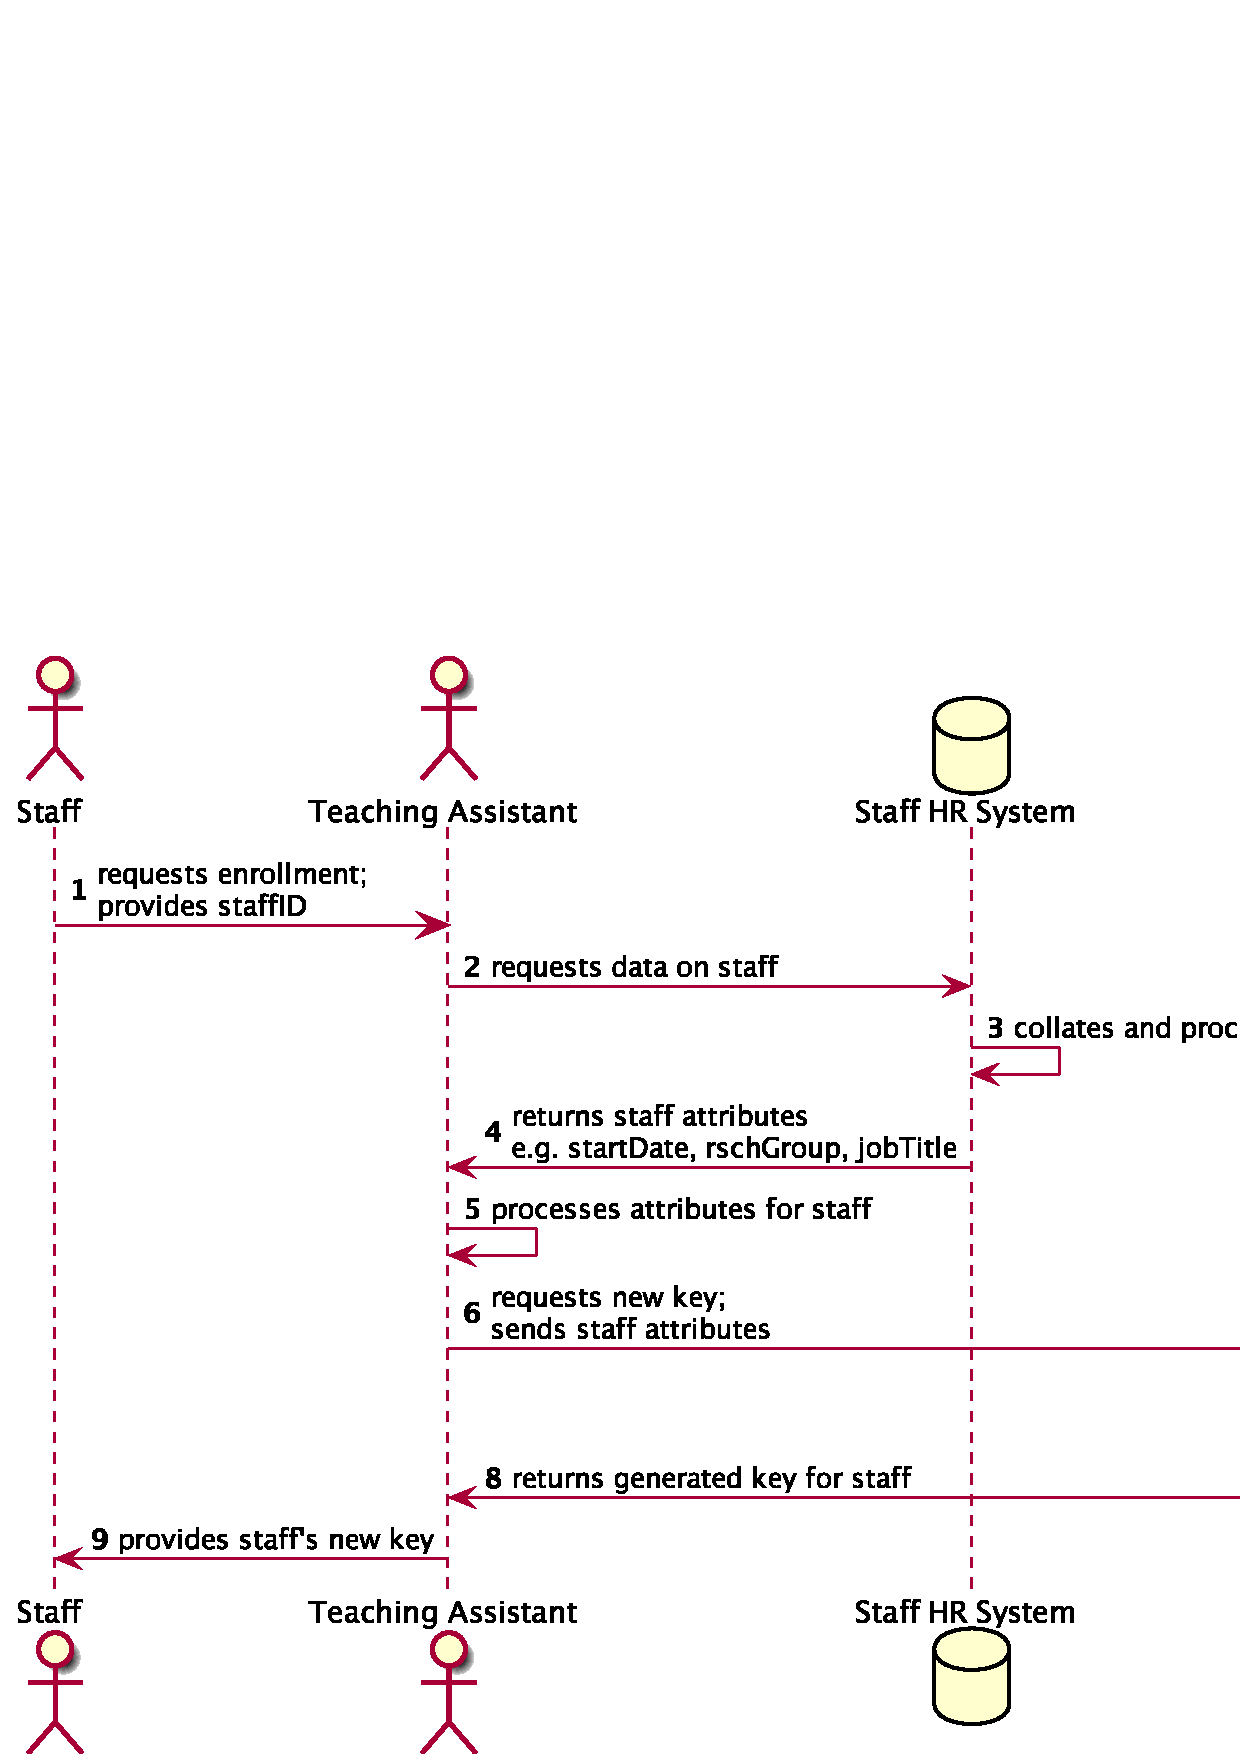
\includegraphics[width=\linewidth,keepaspectratio]{appendices/diagrams/flow_of_info/enrollment_sta_sequence.pdf}

    \caption{A sequence diagram demonstrating the enrolment process for a staff member.}

\end{figure}

\section{Appendix E - System Architecture Diagram}
\label{appendix:architecture_diagram}

\Cref{fig:appendix_sys_arch_full} represents a system architecture diagram for the \theResServer system. This diagram is an alternative to the condensed system architecture diagram in \Cref{fig:sys_arch_abbrv}.

The \acrfull{mks} is shown in an offline state with access to a local copy of the \OpenABE library for provisioning the system \& generating user keys. The \acrfull{prs} is shown receiving offline updates from the \acrshort{mks}, managing a local database with resource metadata \& the associated resource storage and providing search, config and upload \& download interfaces for clients. The \acrfull{crs} is shown with local access to an \OpenABE library for encryption \& decryption and access to an abstract Authentication Service (such as the university's SSO system). The \acrshort{crs} also implements the search, config and upload \& download interfaces provided by the \acrshort{prs} and provides its own upload \& download, encrypt \& decrypt and resource search interfaces for the user.

\begin{figure}[htp]
    \centering
    \label{fig:appendix_sys_arch_full}
    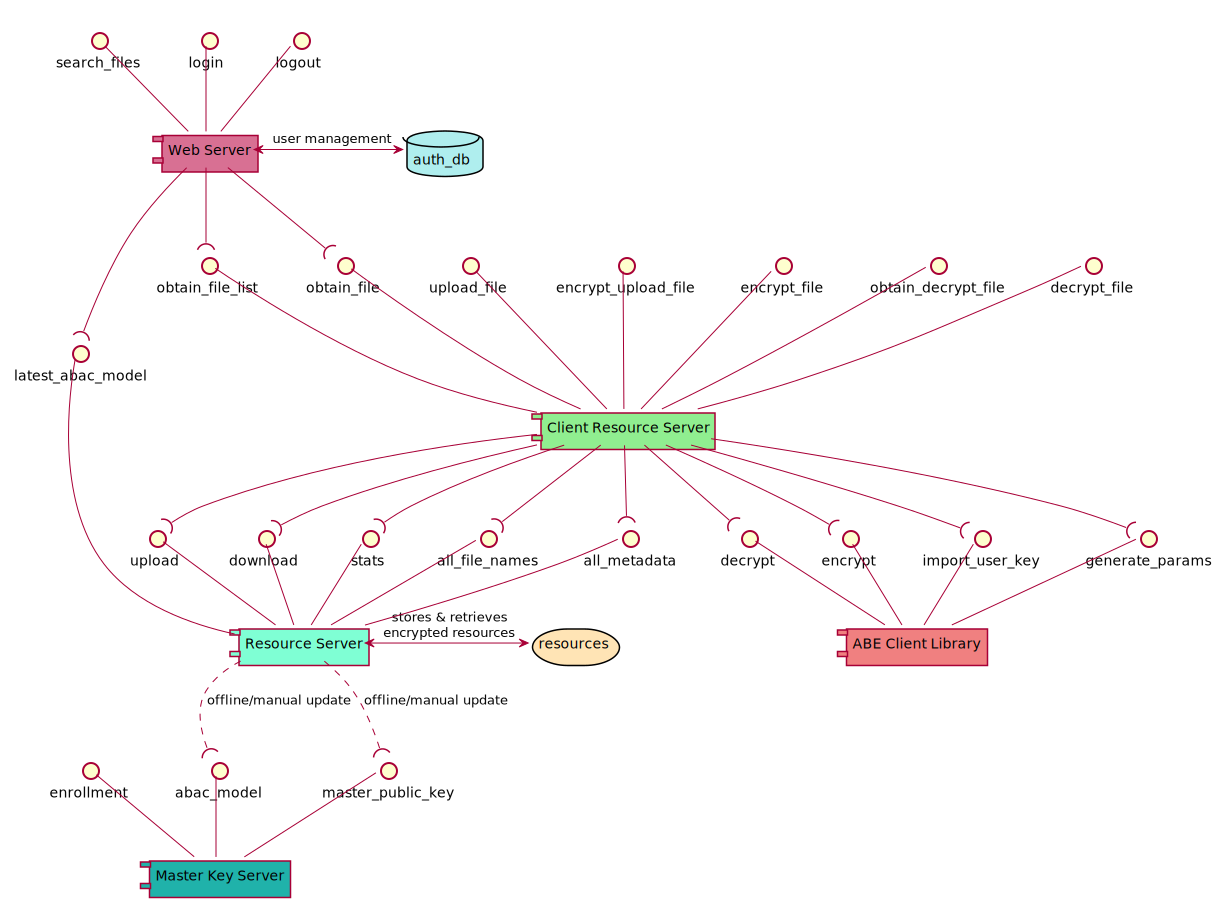
\includegraphics[width=\linewidth,keepaspectratio]{appendices/diagrams/infrastructure/system_architecture.pdf}

    \caption{
      A full architecture diagram describing the system architecture of the \theResServer system.
    }

\end{figure}

\section{Appendix F - Implementing Case Study \#0 with \thePolicyLang}
\label{appendix:case_study_0_policy}

For this study the following details have been assumed:
\begin{itemize}
  \item
    the solutions were encrypted and then uploaded by the Admin staff member
  \item
    the staff member is Teresa Bonner with username `tbonner'
\end{itemize}
\vskip 0.5em
With the details extracted, we can determine the attributes for the policy, where we define \textbf{\textit{Subject} s} and \textbf{\textit{Environment} e} as:
\begin{itemize}
  \item[]
    \textbf{s} $\Rightarrow$ role, accountActiveUntil, username
  \item[]
    \textbf{e} $\Rightarrow$ currentDate
\end{itemize}

Applying the identified attributes for Case Study \#0 (\Cref{subsec:analysis_case_studies_0}) provides the policy in \cref{fig:case_study_policy_0} which would have been embedded in the encrypted lecture slides by the staff member before upload. The encrypted past paper can then remain stored on the server but only accessible to staff members and students.

\begin{figure}[ht]
  \centering
\begin{align*}
  \text{Policy(\textbf{s},\textbf{e})}
  &
    \leftarrow
    \text{username(\textbf{s})} \equiv \text{`tbonner'}
  \\
  &
    \phantom{::}\vee
    \text{role(\textbf{s})} \equiv \text{`Staff'} \mid \text{`Student'}
  \\
  &
    \phantom{::}\wedge
    \text{accountActiveUntil(\textbf{s})} \geq \text{currentDate(\textbf{e})}
\end{align*}
  \caption{
    \label{fig:case_study_policy_0}
    Case Study \#0 policy dictating access to a past exam paper.
    Successful decryption would be possible for the author of the slides (with username `tbonner') \textbf{or} any member of staff \textbf{or} any student. In all cases an active account is also required.
  }
\end{figure}


\section{Appendix G - Implementing Case Study \#2 with \thePolicyLang}
\label{appendix:case_study_2_policy}

For the sake of the scenario, the 1P Programming course was selected with Course Code 1001 as it offers the added complexity of tutors \& demonstrators, but it should be remembered that any course with labs could have been chosen.
\vskip 0.5em
For this study the following details have been assumed:
\begin{itemize}
  \item
    the lab solutions have been uploaded in advance of the actual lab date
  \item
    the lab date is scheduled for 04/12/19
  \item
    the solutions were encrypted and then uploaded by the Lecturer
  \item
    the Lecturer for 1001 is John Williamson with username `jwilliamson'
  \item
    Course 1001 is a Level 1 course
  \item
    Course 1001 has a sister course, 1017
  \item
    the 1P course labs are assisted by tutors \& demonstrators from Level 4+
\end{itemize}

\begin{figure}[ht]
  \centering
\begin{align*}
  \text{Policy($sub$, $env$, $res$)}
  &
    \leftarrow
    \text{username($sub$)} \equiv \text{`jwilliamson'}
  \\
  &
    \phantom{::}\vee
    \text{( role($sub$)} \equiv \text{`Staff'}
  \\
  &
    \phantom{::::::::}\wedge
    \text{jobField($sub$)} \equiv \text{`Research \& Teaching' )}
  \\
  &
    \phantom{::}\vee
    \text{( role($sub$)} \equiv \text{`Student'}
  \\
  &
    \phantom{::::::::}\wedge
    \text{studentLevel($sub$)} \equiv \text{1}
  \\
  &
    \phantom{::::::::}\wedge
    \text{enrolledCourses($sub$)} \equiv \text{[1001, 1017]}
  \\
  &
    \phantom{::::::::}\wedge
    \text{currentDate($env$)} \geq \text{7 December 2019 )}
  \\
  &
    \phantom{::}\vee
    \text{( role($sub$)} \equiv \text{`Student'}
  \\
  &
    \phantom{::::::::}\wedge
    \text{studentLevel($sub$)} \geq \text{4}
  \\
  &
    \phantom{::::::::}\wedge
    \text{studentRole($sub$)} \equiv \text{`Demonstrator UG'} \mid \text{`Demonstrator PG'} \mid \text{`Tutor'}
  \\
  &
    \phantom{::::::::}\wedge
    \text{demonstratorCourses($sub$)} \equiv \text{[1001, 1017]}
  \\
  &
    \phantom{::::::::}\wedge
    \text{startDate($env$)} \leq \text{currentDate($env$)}
  \\
  &
    \phantom{::::::::}\wedge
    \text{endDate($env$)} \geq \text{currentDate($env$) )}
  \\
  &
    \phantom{::}\wedge
    \text{accountActiveUntil($sub$)} \geq \text{currentDate($env$)}
\end{align*}
  \caption{
    \label{fig:case_study_policy_2}
    Case Study \#2 policy dictating access to a set of course `1001' lab solutions.
  }
\end{figure}
Applying the identified attributes for Case Study \#2 provides the policy in \Cref{fig:case_study_policy_2} which would have been embedded in the encrypted lab solution by the Lecturer before upload. The encrypted lab solution can then remain stored on the server but will only accessible to the author of the solutions (with username `jwilliamson') \textbf{or} a member of staff in the `Research \& Teaching' field \textbf{or} a Level 2 student enrolled in the `1001' \& `1017' courses if it is 3 days after the lab date of 04/12/19 \textbf{or} a Level 4+ student employed as a demonstrator or tutor that has been assigned to the `1001' \& `1017' course and it is within their dates of employment. In all cases an active account is also required.


\section{Appendix H - Implementing Case Study \#3 with \thePolicyLang}
\label{appendix:case_study_3_policy}

Applying the identified attributes for Case Study \#3 (\Cref{subsec:analysis_case_studies_3}) provides the policy in \cref{fig:case_study_policy_3} which would have been embedded in the encrypted exam script by the Lecturer before upload. The encrypted exam script can then remain stored on the server but would only be the Lecturer themselves, as well as the specified collaborators.

Further access would be granted to staff members in the Professional, Administrative \& Support field that specifically have the Administration role, as well as Research \& Teaching staff members that belong to the FATA research group and the Programming Languages research theme. Lastly, access would be granted to markers that have been assigned to the 4016 course and will be actively marking during the marking period (12/05/20\textemdash10/06/20).

\begin{figure}[ht]
  \centering
\begin{align*}
  \text{Policy(\textbf{s},\textbf{e})}
  &
    \leftarrow
    \text{username(\textbf{s})} \equiv \text{`odardha'} \mid \text{`sgay'} \mid \text{`jodonnell'}
  \\
  &
    \phantom{::}\vee
    \text{( role(\textbf{s})} \equiv \text{`Staff'}
  \\
  &
    \phantom{::::::::}\wedge
    \text{jobField(\textbf{s})} \equiv \text{`Professional, Administrative \& Support'}
  \\
  &
    \phantom{::::::::}\wedge
    \text{jobRole(\textbf{s})} \equiv \text{`Administration' )}
  \\
  &
    \phantom{::}\vee
    \text{( role(\textbf{s})} \equiv \text{`Staff'}
  \\
  &
    \phantom{::::::::}\wedge
    \text{jobField(\textbf{s})} \equiv \text{`Research \& Teaching'}
  \\
  &
    \phantom{::::::::}\wedge
    \text{researchGroup(\textbf{s})} \equiv \text{`FATA'}
  \\
  &
    \phantom{::::::::}\wedge
    \text{researchTheme(\textbf{s})} \equiv \text{`Programming Languages' )}
  \\
  &
    \phantom{::}\vee
    \text{( role(\textbf{s})} \equiv \text{`Staff'}
  \\
  &
    \phantom{::::::::}\wedge
    \text{staffRole(\textbf{s})} \equiv \text{`Marker'}
  \\
  &
    \phantom{::::::::}\wedge
    \text{markerFrom(\textbf{s})} \geq \text{12 May 2020}
  \\
  &
    \phantom{::::::::}\wedge
    \text{markerTo(\textbf{s})} \leq \text{10 June 2020}
  \\
  &
    \phantom{::::::::}\wedge
    \text{markerCourses(\textbf{s})} \equiv \text{4016}
  \\
  &
    \phantom{::}\wedge
    \text{accountActiveUntil(\textbf{s})} \geq \text{currentDate(\textbf{e})}
\end{align*}
  \caption{
    \label{fig:case_study_policy_3}
    Case Study \#3 policy dictating access to a work-in-progress exam script for course `4016'.
    Successful decryption would be possible for the author of the solutions (with username `odardha') as well as the named collaborators (with usernames `sgay' \& `jodonnell') \textbf{or} for a member of staff in the `Professional, Administrative \& Support' field with the `Administration' role \textbf{or} for a member of staff in the `Research \& Teaching' field that is also in the `FATA' research group and the `Programming Languages' research theme \textbf{or} for a member of staff with the `Marker' role that is assigned to marking duties within the marking period and has been assigned to the `4016' course. In all cases an active account is also required.
  }
\end{figure}


\section{Appendix I - Implementing Case Study \#4 with \thePolicyLang}
\label{appendix:case_study_4_policy}

In this case, the student has encrypted and uploaded their dissertation to the \theResServer system with access to be granted for their supervisor, the assigned reader and additionally, the Project Coordinator.
\vskip 0.5em
For this study the following details have been assumed:
\begin{itemize}
  \item
    the student has the ID and username `2123456z'
  \item
    their supervisor is Quintin Cutts with username `qcutts'
  \item
    their assigned reader is Paul Siebert with username `psiebert'
  \item
    the Project Coordinator is John Williamson with username `jwilliamson'
\end{itemize}

\begin{figure}[ht]
  \centering
\begin{align*}
  \text{Policy($sub$, $env$, $res$)}
  &
    \leftarrow
    \text{( role($sub$)} \equiv \text{`Student'}
  \\
  &
    \phantom{::::::}\wedge
    \text{username($sub$)} \equiv \text{`2123456z' )}
  \\
  &
    \phantom{::}\vee
    \text{( role($sub$)} \equiv \text{`Staff'}
  \\
  &
    \phantom{::::::}\wedge
    \text{username($sub$)} \equiv \text{`qcutts'} \mid \text{`psiebert'} \mid \text{`jwilliamson' )}
  \\
  &
    \phantom{::}\wedge
    \text{accountActiveUntil($sub$)} \geq \text{currentDate($env$)}
\end{align*}
  \caption{
    \label{fig:case_study_policy_4}
    Case Study \#4 policy dictating access to a completed dissertation.
  }
\end{figure}
Applying the identified attributes for Case Study \#4 provides the policy in \Cref{fig:case_study_policy_4} which would have been embedded in the encrypted dissertation by the student before upload. The encrypted dissertation can then remain stored on the server but only accessible to the student (with username `2123456z') and the three identified staff members (with usernames `qcutts', `psiebert', `jwilliamson'). In all cases an active account is also required.


\section{Appendix J - Physical Assets for Master Key Server}
\label{appendix:mks_assets}

\begin{table}[htp]
  \rowcolors{2}{}{gray!3}
  \begin{tabularx}{\linewidth}{lX}
    \textbf{Asset}          & \textbf{Description} \\
    Router or Switch        &	Router (AP) or Switch host is connected to (if host is not offline). \\
    Network connection      &	Physical connection to network (if host not offline). \\
    Storage                 &	Storage for host, high risk, contains keys, config, server files etc. \\
    Monitor                 &	General output for host, low risk. \\
    Keyboard                &	General input for host, low risk. \\
    Mouse                   &	General input for host, low risk. \\
    Computer                &	The actual host machine of the server. \\
    Room key                &	Simply the key that grants access to the physical room the server is located in. \\
    Building                &	The physical building the host machine is located in. \\
    Room                    &	The physical room the host machine is located in. \\
    External Storage/Media  &	Any external storage/media attached to the host machine during operation. \\
  \end{tabularx}
  \caption{Physical assets for the \acrfull{mks}}
  \label{tab:physical_assets_mk}
\end{table}

\section{Appendix K - Assets for Public Resource Server}
\label{appendix:prs_assets}

\begin{table}[htp]
  \rowcolors{2}{}{gray!3}
  \begin{tabularx}{\linewidth}{lX}
    \textbf{Asset}            & \textbf{Description} \\
    Master Public Key file    &	Not dangerous, value is distributed as part of normal operation. \\
    Global Attributes file    &	As above, is distributed as part of normal operation but potentially reveals information on the system. \\
    Server Secret (sessions)  &	Secret used to set up sessions with users, and generate CSRF tokens. Potentially dangerous. \\
    Local web server files    &	Contains other config files, but also the key files. Needs protection. \\
    jinja2 plugin             &	Plugin to generate templates. Lowish risk, but an external party provides software. \\
    flask plugin              &	Tool to create and run a web server, potentially damaging. Produced and updated by an external party. \\
    PyMongo plugin            &	Plugin used by flask server to communicate with the Mongo DB. \\
    Python3 lib               &	The Python3 library. Similar to above, lower vulnerability as very openly and globally reviewed. \\
    MongoDB Database          & Database of resource meta data. \\
    MongoDB system            & System running MongoDB databases. Produced and updated by an external party. \\
    C lib                     &	The C library. Similar to Python, low vulnerability as extremely openly and globally reviewed. Slow to update as well. \\
    Resource files            & Encrypted ciphertexts representing the resources stored on the server. \\
    Firewall                  &	Firewall of the host. Should block incoming requests. May not even be necessary as Key Server should be offline when deployed. \\
    UNIX OS                   &	The UNIX OS the host is running on. External party software so potential risk.
  \end{tabularx}
  \caption{Virtual assets for the \acrfull{prs}}
  \label{tab:virtual_assets_pr}
\end{table}

\begin{table}[htp]
  \rowcolors{2}{}{gray!3}
  \begin{tabularx}{\linewidth}{lX}
    \textbf{Asset}          & \textbf{Description} \\
    Router or Switch        &	Router (AP) or Switch host is connected to. \\
    Network connection      &	Physical connection to network. \\
    Storage                 &	Storage for host, high risk, contains resources, config, server files etc. \\
    Computer                &	The actual host machine of the server. \\
    Building                &	The physical building the host machine is located in. \\
    Room                    &	The physical room the host machine is located in. \\
    External Storage/Media  &	Any external storage/media attached to the host machine during operation. \\
  \end{tabularx}
  \caption{Physical assets for the \acrfull{prs}}
  \label{tab:physical_assets_pr}
\end{table}

\section{Appendix L - Assets for Client Resource Server}
\label{appendix:crs_assets}

\begin{table}[htp]
  \rowcolors{2}{}{gray!3}
  \begin{tabularx}{\linewidth}{lX}
    \textbf{Asset}            & \textbf{Description} \\
    User Key                  & High risk. The end user's private key, used to decrypt all resources. \\
    Master Public Key file    &	Not dangerous, value is distributed as part of normal operation. \\
    Global Attributes file    &	As above, is distributed as part of normal operation but potentially reveals information on the system. \\
    Server Secret (sessions)  &	Secret used to set up sessions with users, and generate CSRF tokens. Potentially dangerous. \\
    Local web server files    &	Contains other config files, but also the key files. Needs protection. \\
    jinja2 plugin             &	Plugin to generate templates. Lowish risk, but an external party provides software. \\
    flask plugin              &	Tool to create and run a web server, potentially damaging. Produced and updated by an external party. \\
    PyMongo plugin            &	Plugin used by flask server to communicate with the Mongo DB. \\
    PyOpenABE bindings        &	Python bindings for decryption. High risk. Also maintained by external party. \\
    cython lib/plugin         &	Python tool to compile python down to C. Interprets all bindings. So as above. \\
    Python3 lib               &	The Python3 library. Similar to above, lower vulnerability as very openly and globally reviewed. \\
    OpenABE C lib             &	OpenABE library for all user key generation. High risk. Maintained by external party. \\
    MongoDB Database          & Database of resource meta data. \\
    MongoDB system            & System running MongoDB databases. Produced and updated by an external party. \\
    C lib                     &	The C library. Similar to Python, low vulnerability as extremely openly and globally reviewed. Slow to update as well. \\
    Resource files            & Decrypted resources downloaded from server. \\
    Firewall                  &	Firewall of the host. Up to user. \\
    UNIX OS                   &	The UNIX OS the host is running on. External party software so potential risk.
  \end{tabularx}
  \caption{Virtual assets for the \acrfull{crs}}
  \label{tab:virtual_assets_cr}
\end{table}

\begin{table}[htp]
  \rowcolors{2}{}{gray!3}
  \begin{tabularx}{\linewidth}{lX}
    \textbf{Asset}          & \textbf{Description} \\
    Router or Switch        &	Router (AP) or Switch host is connected to (if host is not offline). \\
    Network connection      &	Physical connection to network (if host not offline). \\
    Storage                 &	Storage for host, high risk, contains keys, config, server files etc. \\
    Monitor                 &	General output for host, low risk. \\
    Keyboard                &	General input for host, low risk. \\
    Mouse                   &	General input for host, low risk. \\
    Computer                &	The actual host machine of the server. \\
    External Storage/Media  &	Any external storage/media attached to the host machine during operation. \\
  \end{tabularx}
  \caption{Physical assets for the \acrfull{crs}}
  \label{tab:physical_assets_cr}
\end{table}

\section{Electronic Appendices}
\label{appendix:electronic_appendices}

\subsection{Appendix E1 - Deployment Roles \& Users}
\label{appendix:e_roles_users}

We make note of the Deployment Roles \& Users mind map document. Although contained in Appendix \ref{appendix:roles_users}, it is too large to be viewed fully within the dissertation, therefore it is included in the submitted code file under: \texttt{l4-project-research/Mind\_Maps/ABE\_Users.slides\_Oct26.pdf}.

\subsection{Appendix E2 - Environment Attributes}
\label{appendix:e_environments}

We make note of the Environment Attributes mind map document. Although contained in Appendix \ref{appendix:environments}, it is too large to be viewed fully within the dissertation, therefore it is included in the submitted code file under: \texttt{l4-project-research/Mind\_Maps/ABE\_Environments.slides\_Oct26.pdf}.

\subsection{Appendix E3 - System Use Cases}
\label{appendix:e_use_cases}

We make note of the system Use Cases mind map document. Although contained in Appendix \ref{appendix:use_cases}, it is too large to be viewed fully within the dissertation, therefore it is included in the submitted code file under: \texttt{l4-project-research/Mind\_Maps/ABE\_Use\_Cases.slides\_Oct26.pdf}.

\subsection{Appendix E4 - Risk Assessment}
\label{appendix:e_risk_assessment}

We make note of the Risk Assessment Excel document. Too large to submit within the dissertation, it is included in the submitted code file under: \texttt{l4-project-research/reports/RiskAssessment.xlsx}.

\end{appendices}
